% !TeX encoding = UTF-8
% !TeX spellcheck = es_ES
% !TeX root = DccPowerDistribution.tex

La placa DccPowerDistribution tiene una serie de jumpers y puntos de soldaura/corte
que permiten cambiar ciertas partes y ajustar su comportamiento.

\subsection{Jack o Terminal Atornillable}

El conector Jack se puede conectar directamente a un adaptador AC/DC que tenga salida 
jack 2mm, un conector muy generico usado por diferentes dispositivos electronicos.
Por norma general, solo tienen una salida, por lo que solo se puede conectar a una placa

Por otra parte el terminal Atornillable facilita la conexion cuando ya existe un bus de
corriente continua CC. Con lo que es mas facil conectar varias placas.

Ambos estan conectados en paralelo sin ninguna proteccion, por lo que es necesario
asegurarse que solo uno recibe corriente. La forma más sencilla es solo soldar uno 
de ellos o conectar solo uno.

\begin{figure}[H]
    \centering
    \begin{minipage}{0.25\textwidth}
        \centering
        \begin{tikzpicture}
    
    
    \pic[rotate=-90,transform shape](ac) at(-1,0) {WallAc};
    \pic[rotate=-90,transform shape](board)at (1,0) {SmallBoard};

    \draw[red, line width=4pt,rounded corners=6pt] (ac-jack.center) 
    -- (ac-jack.center |- 0,1.8) 
    -- (board-jack.center|- 0,1.8) 
    -- (board-jack.center);
    %\draw[green] (ac-mains.center) -- (board-terminal.center);

\end{tikzpicture} 
        \caption{Solo Jack}
        \label{fig:VccConnectionJack}
    \end{minipage}
    \hfill
    \begin{minipage}{0.7\textwidth}
        \centering
        \begin{tikzpicture}

    \pic[rotate=-90,transform shape](ac) at(-3,0) {WallAc};
    \pic[rotate=-90,transform shape](board1)at (-1,0) {SmallBoard};
    \pic[rotate=-90,transform shape](board2)at (1,0) {SmallBoard};
    \pic[rotate=-90,transform shape](board3)at (3,0) {SmallBoard};


    \begin{scope}[shift={(5,0)}]
        \draw[black] (-0.7,-1.3) rectangle +(1.4,2.6);
        \node[] at (0,0.3) {Otro};
        \node[] at (0,-0.3) {Modulo};
    \end{scope}

    \draw[red!75, line width=2pt,rounded corners=6pt] (0,1.8)
    --(board1-terminal.center -| 0,0)
    --(board1-terminal.center);
    
    \draw[red!75, line width=2pt,rounded corners=6pt] (2,1.8)
    --(board2-terminal.center -| 2,0)
    --(board2-terminal.center);
    
    \draw[red!75, line width=2pt,rounded corners=6pt] (4,1.8)
    --(board3-terminal.center -| 4,0)
    --(board3-terminal.center);

    \draw[red!75, line width=2pt,rounded corners=6pt] (6,1.8)
    --(board2-terminal.center -| 6,0)
    --(board2-terminal.center -| 5.7,0);


    % Bus
    \draw[red, line width=4pt,rounded corners=6pt] (ac-jack.center) 
    -- (ac-jack.center |- 0,1.8)
    -- (6.5,1.8);
\end{tikzpicture} 
        \caption{Solo Terminal}
        \label{fig:VccConnectionTerminal}
    \end{minipage}
\end{figure}

Si se sueldan los dos conectores se puede usar una placa como iniciador de bus CC

\begin{figure}[H]
    \centering
    \begin{tikzpicture}
    
    
    \pic[rotate=-90,transform shape](ac) at(-3,0.5) {WallAc};
    \pic[rotate=-90,transform shape](board1)at (-1,0.5) {SmallBoard};

    \draw[red, line width=4pt,rounded corners=6pt] (ac-jack.center) 
    -- (ac-jack.center |- 0,2.8) 
    -- (board1-jack.center|- 0,2.8) 
    -- (board1-jack.center);

    \pic[rotate=-90,transform shape](board2)at (1,-0.5) {SmallBoard};
    \pic[rotate=-90,transform shape](board3)at (3,-0.5) {SmallBoard};
    
    \begin{scope}[shift={(5,-0.5)}]
        \draw[black] (-0.7,-1.3) rectangle +(1.4,2.6);
        \node[] at (0,0.3) {Otro};
        \node[] at (0,-0.3) {Modulo};
    \end{scope}
    
    \draw[red!75, line width=2pt,rounded corners=6pt] (board1-terminal.center -| 2,1.8)
    --(board2-terminal.center -| 2,0)
    --(board2-terminal.center);
    
    \draw[red!75, line width=2pt,rounded corners=6pt] (board1-terminal.center -| 4,1.8)
    --(board3-terminal.center -| 4,0)
    --(board3-terminal.center);

    \draw[red!75, line width=2pt,rounded corners=6pt] (board1-terminal.center -| 6,1.8)
    --(board2-terminal.center -| 6,0)
    --(board2-terminal.center -| 5.7,0);


    % Bus
    \draw[red, line width=4pt,rounded corners=6pt] (board1-terminal.center)
        -- (board1-terminal.center -| 6.5,1.8);
    %\draw[green] (ac-mains.center) -- (board-terminal.center);

\end{tikzpicture} 
    \caption{Jack Iniciando Bus}
    \label{fig:VccConnectionJackBus}
\end{figure}

En el caso de que se use un bus de Coriente Continua, es posible añadir modulos que no sean
de la gama DccDiyTools, pero es necesario asegurarse de que sean compatibles a nivel de voltaje
y que el adaptador de corriente sea capaz de suministrar la corriente necesaria para todos los
modulos conectados.

\subsection{Origen Automatico, siempre DCC o siempre CC}
La corriente puede ser tomada desde el bus DCC o un bus de Corriente Continua (CC).
Esto se puede hacer mediante la activacion de los ByPass, o lineas azules en el diagrama
de bloques. El selector principal que determina el origen es J3 y tiene tres opciones

\begin{figure}[H]
    \centering
    \begin{tikzpicture}
    \begin{scope}[shift={(-4,0)}]

        \begin{scope}
            \clip (-1,-2) rectangle  +(2,4);

            \node[inner sep=0pt] at (5.6,-0.)
                {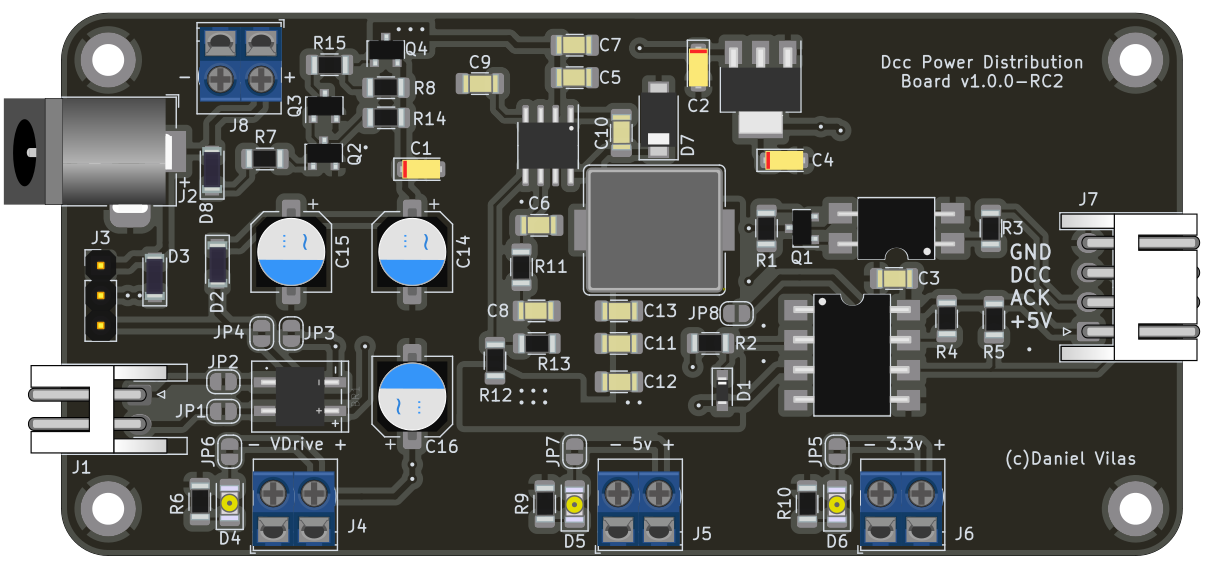
\includegraphics[scale=1.3]{images/front.png}};
        \end{scope}
        \draw[yellow,line width=2pt,rounded corners=4pt] 
            (-0.3,-0.7) rectangle +(0.6,1.4);
        \node[below] at (0,-2) {(a) Automatico};
    \end{scope}

    \begin{scope}
        % \draw [step=0.1,very thin, yellow] (-2,-2) grid (2,2);
        % \draw [step=0.5,very thin, red] (-2,-2) grid (2,2);
        % \draw [very thin, green] (-2,-2) grid (2,2);

        \begin{scope}
            \clip (-1,-2) rectangle  +(2,4);

            \node[inner sep=0pt] at (5.6,-0.)
                {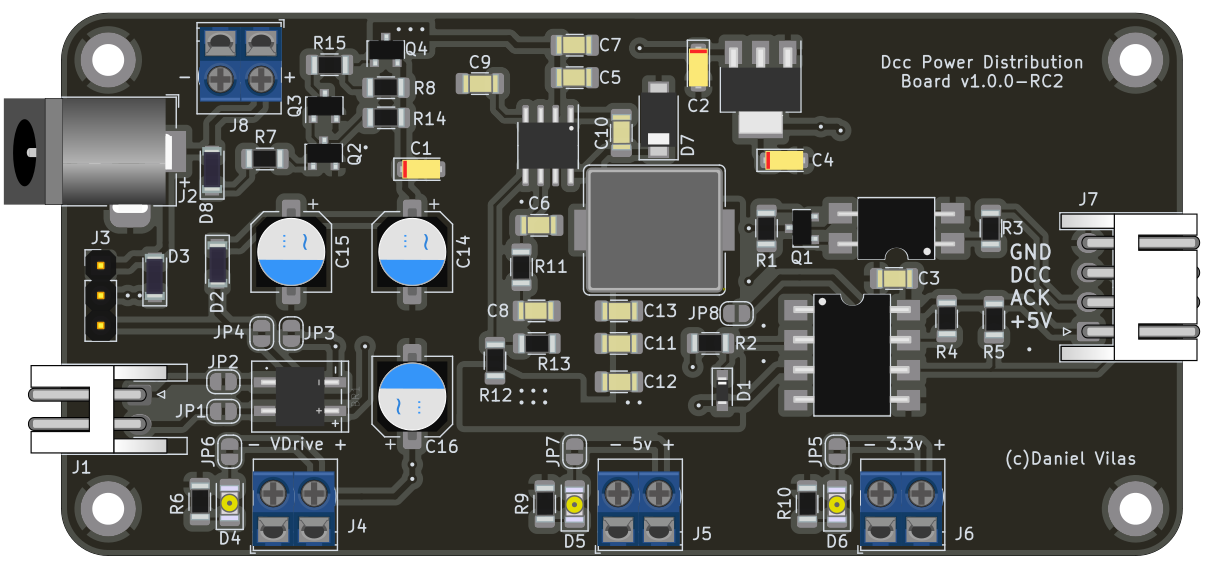
\includegraphics[scale=1.3]{images/front.png}};
        \end{scope}
        %\draw [step=0.1,very thin, yellow] (-0.5,-1) grid +(1,2);
        \draw[yellow,line width=2pt,rounded corners=4pt] 
            (-0.3,-0.7) rectangle +(0.6,1.4);
        \draw[blue, fill=blue!75,line width=1pt]
            (-0.2,0.4) rectangle +(0.35,-.65); 
        \node[below] at (0,-2) {(b) Corriente Continua};
    \end{scope}

    \begin{scope}[shift={(4,0)}]

        \begin{scope}
            \clip (-1,-2) rectangle  +(2,4);

            \node[inner sep=0pt] at (5.6,-0.)
                {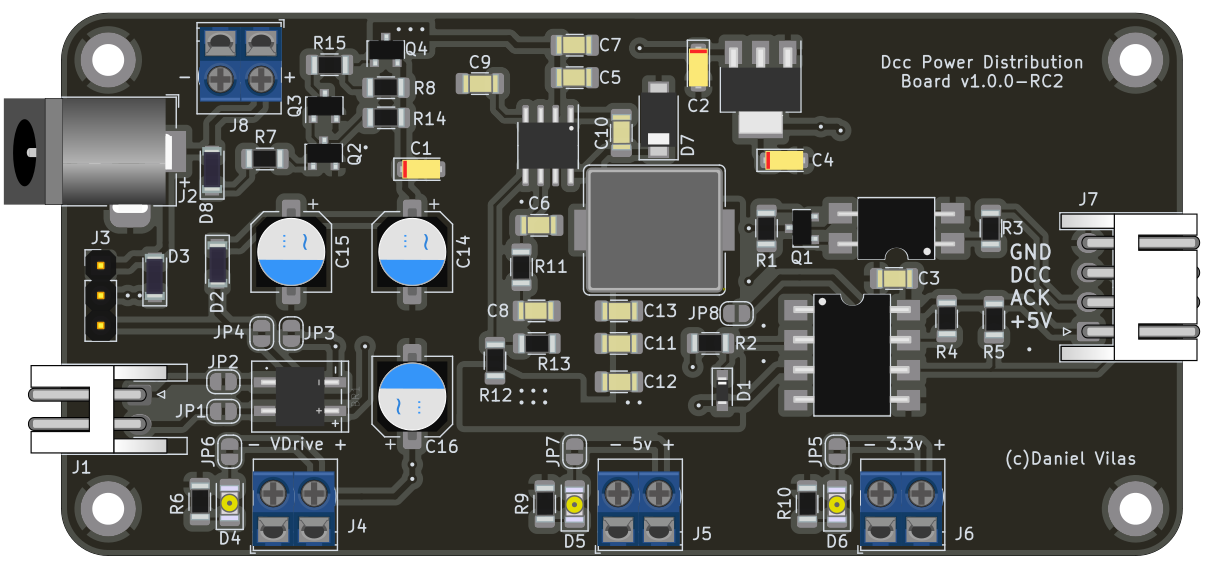
\includegraphics[scale=1.3]{images/front.png}};
        \end{scope}
        %\draw [step=0.1,very thin, yellow] (-0.5,-1) grid +(1,2);
        
        \draw[yellow,line width=2pt,rounded corners=4pt] 
            (-0.3,-0.7) rectangle +(0.6,1.4);

        \draw[blue, fill=blue!75,line width=1pt]
        (-0.2,0.05) rectangle +(0.35,-.65); 
        \node[below] at (0,-2) {(c) DCC};
    \end{scope}
\end{tikzpicture}
    \caption{Opciones J3 - Origen de corriente}
    \label{fig:VccSelection}
\end{figure}

J3 por defecto vendra sin componente, para que se pueda soldar un cable en la configuracion desada
y ademas pueda servir como puntos  de prueba. Puede ponerse una cabezera dupont 2.54mm y asi usar 
jumpers.

\begin{itemize}
    \item \textbf{Automatico}: Dejar J3 sin conectar nada.
    \item \textbf{Siempre CC}: Pone un jumer entre los pines más cercanos al Jack CC.
    \begin{itemize}
        \item En esta configuracion se recomienda desactivar la señal DCC, no conectandola
 o mediante \textbf{JP1, JP2, JP3 y JP4}.
        \item Con esta configuracion se puede lograr un maximo de \textbf{3A}. Pero simpre y
cuando se suelde un cable entre los puntos \sidenote[][-1em]{Hay jumpers de \textbf{3A}, en ese caso se pueden usar}.             
    \end{itemize}
     \item \textbf{Siempre DCC}:Pone un jumer entre los pines más cercanos al conector DCC.
     \begin{itemize}
         \item En esta configuracion se recomienda no conectar corriente CC
         \item Con esta configuracion se puede lograr un maximo de \textbf{2A}. Pero simpre y
 cuando se suelde un cable entre los puntos.             
     \end{itemize}
\end{itemize}

\subsection{Desactivacion Entrada de corriente DCC}
Es posible configurar DccPowerDistribution para que sea imposible utilizar la señal DCC como
entrada de corriente, y no perder la señal DCC-TTL. Para ello se pueden utilizar los puntos
de soldadura \textbf{JP1, JP2, JP3} y \textbf{JP4}.


\begin{figure}[H]
    \centering
    \begin{tikzpicture}
    \begin{scope}[shift={(-2,0)}]
        % \draw [step=0.1,very thin, yellow] (-2,-2) grid (2,2);
        % \draw [step=0.5,very thin, red] (-2,-2) grid (2,2);
        % \draw [very thin, green] (-2,-2) grid (2,2);
        \begin{scope}
            \clip (-1.8,-1.5) rectangle  +(3.6,3);
            \node[inner sep=0pt] at (4.7,1.5)
                {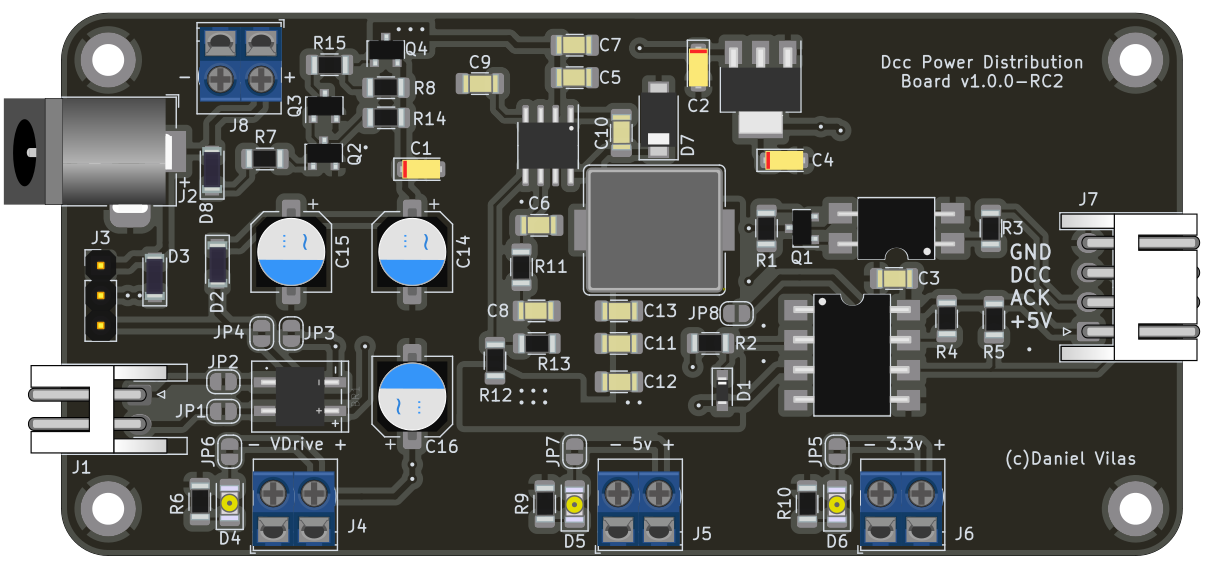
\includegraphics[scale=1.3]{images/front.png}};
        \end{scope}
        \draw[yellow,line width=2pt,rounded corners=4pt] 
            (-0.2,-0.1) rectangle +(1,0.95);
        
            \node[below] at (0,-2) {(a) JP1 y JP2};

        %\draw[white] (-2,0)--(2,0);
    \end{scope}
    \begin{scope}[shift={(3,0)}]
        % \draw [step=0.1,very thin, yellow] (-2,-2) grid (2,2);
        % \draw [step=0.5,very thin, red] (-2,-2) grid (2,2);
        % \draw [very thin, green] (-2,-2) grid (2,2);
        \begin{scope}
            \clip (-1.8,-1.5) rectangle  +(3.6,3);
            \node[inner sep=0pt] at (4.7,1.5)
                {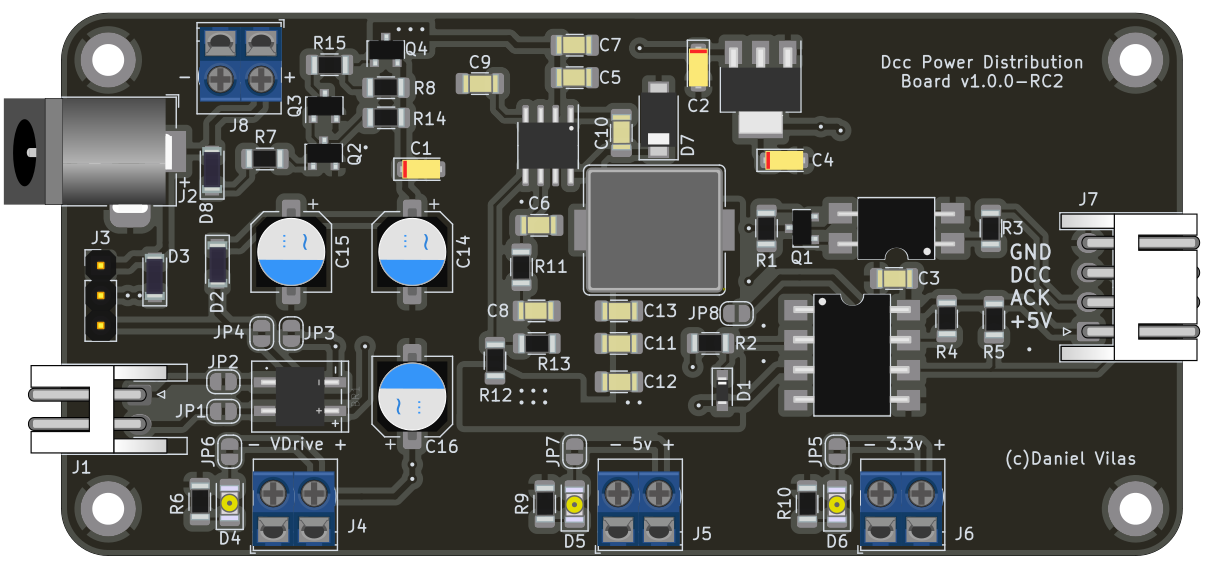
\includegraphics[scale=1.3]{images/front.png}};
        \end{scope}
        \draw[yellow,line width=2pt,rounded corners=4pt] 
            (0.25,0.7) rectangle +(1.5,0.55);
        
            \node[below] at (0,-2) {(b) JP3 y JP4};

        %\draw[white] (-2,0)--(2,0);
    \end{scope}
\end{tikzpicture}
    \caption{Ubicacion DCC Disable}
    \label{fig:DccDisable}
\end{figure}

Como se puede ver hay dos juegos de puntos de soldadura, JP1 con JP2 y JP3 con JP4. Cada juego
realiza una funcion diferente.
\begin{itemize}
    \item \textbf{JP1} y \textbf{JP2}: conectan la señal DCC al bloque rectificador. Si se cortan
se pierde la funcionalidad ACK y la entrada de corriente por DCC. Se ha detectado que las centrales
DCC pueden confundirse con el bloque rectificador\sidenote[][-3em]{Tiene que ver con el tiempo de recuparacion
de los diodos} y suponer que hay un corto\sidenote[][1em]{Se han utilizado rectificadores 
rapidos, por lo que no se espera que suceda esto}. En estas centrales
es necesario cortar estos puntos de soldadura.
    \item \textbf{JP3} y \textbf{JP4}: conectan la señal rectificada DCC al bloque de proteccion.
    Se deben cortar ambos para desactivar la corriente DCC y aun mantener la funcionalidad ACK
        
\end{itemize}

\subsection{DCC +5V}
Para que la salida DCC-TTL funcione se necesita una señal de referencia TTL. La interface DCC hace un
Pull-Up a este valor cuando no hay señal DCC y lo situara a 0v conforme la señal vaya recibiendose.
Este valor de referencia puede ser el mismo carrill 5V generado por DccPowerDistribution, o venir de
fuera mediante el pin DCC \textbf{+5V}.

\begin{figure}[H]
    \centering
    \begin{tikzpicture}
    \begin{scope}
        \clip (-2,-2) rectangle  + (4,4);
        %\draw [very thin, green, fill=yellow]  (-6,-4) rectangle (12,8);
        \node[inner sep=0pt] (russell) at (-8.1,0)
            {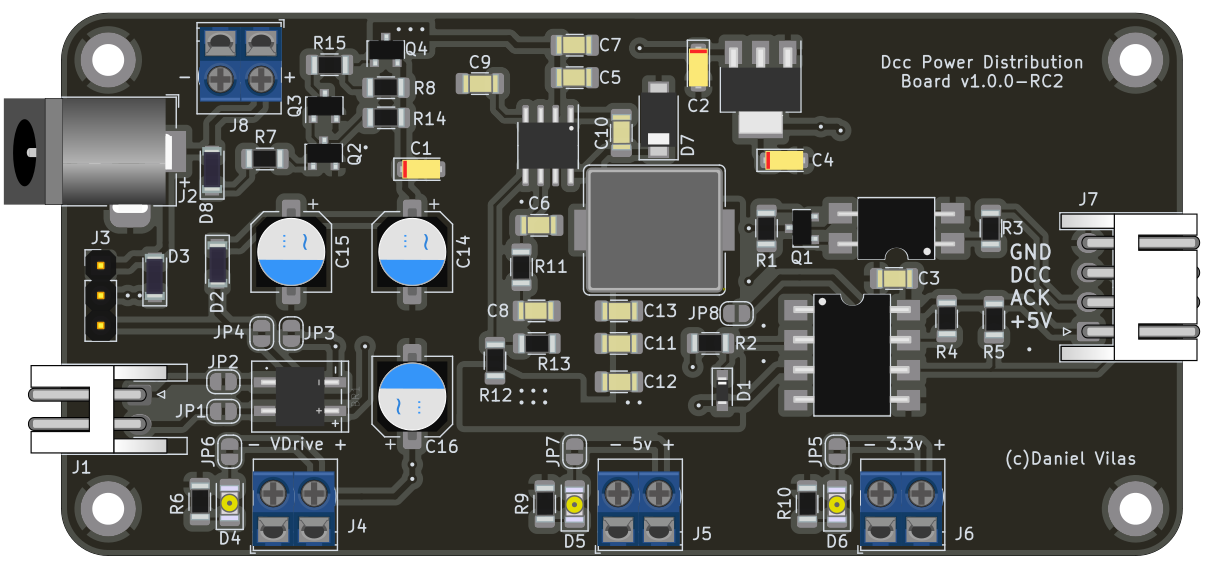
\includegraphics[scale=2]{images/front.png}};
        %\draw [very thin, green]  (-7,-3) grid (6,4);
    \end{scope}
    %\draw [very thin, green] (-3,-2) grid (3,2);
    \draw [color=yellow,line width=2pt](-1.6,-0.9) rectangle + (1.6,1.8);
    
    \node[right] at (4,1) {GND: Ref 0V};
    \node[right] at (4,0.33) {DCC-TTL: Salida Señal DCC};
    \node[right] at (4,-0.33) {ACK: Entrada Señal ACK};
    \node[right] at (4,-1) {+5V: Entrada/Salida Ref TTL};
    
    \draw [color=black, line width=3pt,cap=round] (2.0,0.75) -- (4,1);
    \draw [color=blue, line width=3pt,cap=round] (2,0.25) -- (4,0.33);
    \draw [color=orange, line width=3pt,cap=round] (2,-0.25) -- (4,-0.33);
    \draw [color=red, line width=3pt,cap=round] (2.0,-0.75) -- (4,-1);
\end{tikzpicture}
    \caption{Entrada/Salida Señal DCC}
    \label{fig:DccOut2}
\end{figure}

Se puede cambiar este comportamiento mediante el punto de soldadura \textbf{JP8}.

\begin{figure}[H]
    \centering
    \begin{tikzpicture}

    %\draw [very thin, green]  (-6,-3) grid (6,3);

    \begin{scope}[shift={(3.4,0)}]
        \pic[scale=2,transform shape] at (-5,0) {SmallBoard}; 
        \begin{scope}
            \clip (-1.5,-1.5) rectangle  +(3,3);
            \node[inner sep=0pt] at (-1,0.45)
                {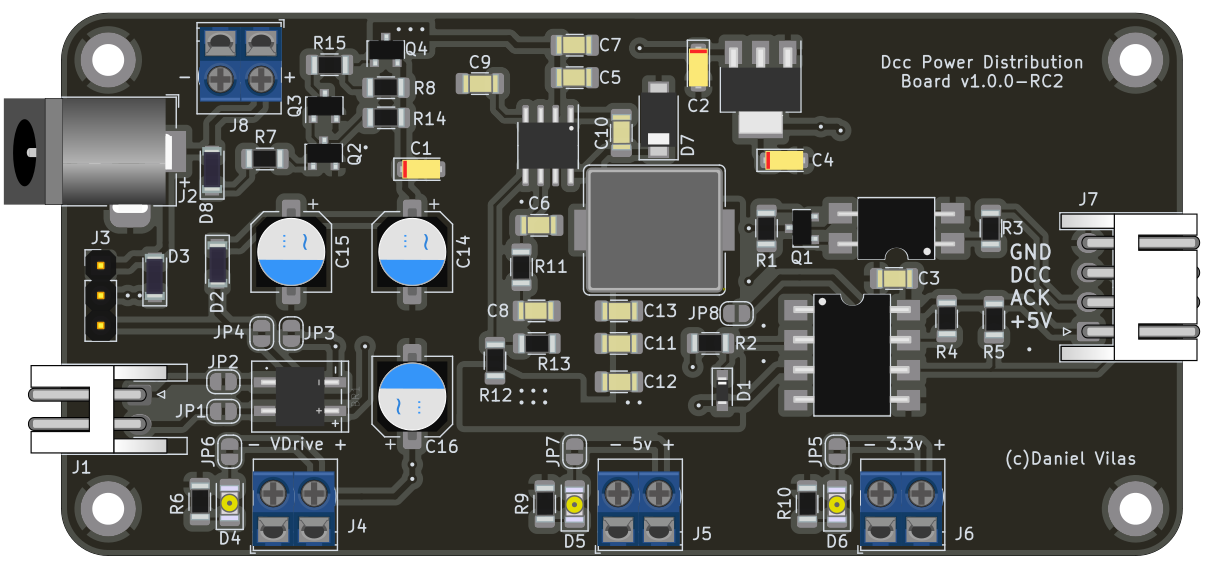
\includegraphics[scale=2]{images/front.png}};
        \end{scope}
        \draw[green, line width=2pt,rounded corners=4pt](-1.6,-1.6) rectangle  +(3.2,3.2);

        \draw[yellow,line width=2pt,rounded corners=4pt] 
            (0.2,-0.25) rectangle +(1.4,0.55);
        %\draw[green] (-8.7,-1.6) rectangle+(10.6,3.2);
        \node(lupaDown) at (-1.5,-1.6){};
        \node(lupaUp) at (-1.5,1.6){};
    \end{scope}
    \draw[green,rounded corners=1pt] (-1.72,-0.48) rectangle+(0.75,0.75);
    \draw[green, line width=1pt, cap=round] (-1.7,-0.48) -- (lupaDown.center);
    \draw[green, line width=1pt, cap=round] (-1.7,0.27) -- (lupaUp.center);
    \draw[yellow,rounded corners=1pt] (-1.3,-0.18) rectangle+(0.35,0.15);
    
\end{tikzpicture}
    \caption{Ubicacion JP8}
    \label{fig:Jp8Loc}
\end{figure}

Si las conexiones estan cortadas el pin DCC +5V se comportara como entrada, requirendo que se suministre
el voltaje de referencia TTL para la salida DCC-TTL. En este caso se puede usar logica 3.3V

Por otra parte, si se unen mediante soldadura. La linea DCC +5V estara conectada al rail +5V generado
por el conversor Buck. Por lo que se puede usar para suministrar corriente a los modulos DCC.

\subsection{Leds de los Railes}
Los Leds junto a los terminales de salida se pueden desconectar para ahorrar unos 
miliamperios de comsumo. Estos leds son utiles para ver de un vistazo rapido el estado
de cada carril de potencia. Pero una vez instalado bajo una maqueta no se van ver siempre
por lo que puede ser interesante desactivarlos.

Cada cada carril tiene asociado un led, un color\sidenote[][]{Puede variar segun ediciones de
DccPowerDistribution}, un Punto de soldadura y una resistencia para limitar su consumo.
El diseño original se recoge en la siguiente tabla:

\begin{table}[H]
    \centering
    \renewcommand\theadfont{\bfseries}
    \setlength{\tabcolsep}{10pt}
    \renewcommand{\arraystretch}{1.5}
    \begin{tabular}{c |c |c |c |c |}
        Carril & \thead[b]{Punto} & \thead[b]{Color($V_{drop}$)} & \thead[b]{Resistencia} & \thead[b]{Consumo} \\ 
        \Xhline{5\arrayrulewidth}
%VDrive
        \rowcolor{Melon!15} Vdrive(12V)
        & JP6 &Blanco(3V) & 900$\Omega$ & 10mA \\
        \hline
        \rowcolor{blue!15} 5V
        & JP7 & Azul(3V) & 200$\Omega$ & 10mA \\
        \rowcolor{cyan!15} 3.3V
        & JP5 & Cyan(2.7V) & 100$\Omega$ & 5.5mA \\
        \hline
    \end{tabular}
    \caption{Diseño de los leds}
    \label{tab:leds}
\end{table}

Junto a cada terminal de salida esta el led, la resitencia y el punto de soldadura.

\begin{figure}[H]
    \centering
    \begin{tikzpicture}[scale=1]
    \begin{scope}
        \clip (-7.,0) rectangle  +(14,2.5);
        \node[inner sep=0pt] (russell) at (0.6,4.75)
            {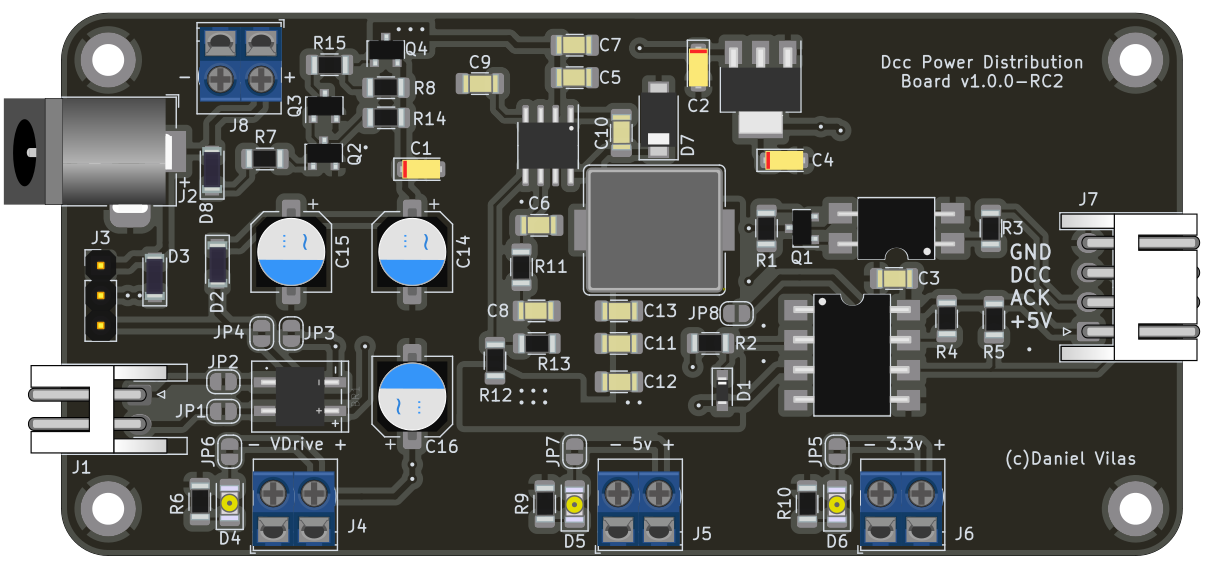
\includegraphics[scale=2]{images/front.png}};
    \end{scope}
    \node [text width = 1.3cm] at (-5,-0.5){VDrive};
    \node [text width = 1.3cm] at (1,-0.5){+5V};
    \node [text width = 1.3cm] at (5.4,-0.5){+3.3V};


    \draw [color= yellow, line width=2pt,rounded corners=2pt] (-6.5,1.5) rectangle +(1.,0.9);
    \draw [color= yellow, line width=2pt,rounded corners=2pt] (-0.6,1.5) rectangle +(1.,0.9);
    \draw [color= yellow, line width=2pt,rounded corners=2pt] (3.8,1.5) rectangle +(1.,0.9);
   
\end{tikzpicture}
    \caption{Ubicacion JP5, JP6 and JP7}
    \label{fig:LedDisable}
\end{figure}

Para deshabilitar un led solo es necesario cortar el punto de soldadura  que corresponda.
Y volverlo a soldar para habilitarlo

\subsection{Cortar y recuperar un punto de soldadura}
Los puntos de soldadura son dos Pads cercanos que pueden estar unidos con una pista entre
ambos, sindo NC o Normally Closed, pero tambien puede estar sin conexion, llamandose NO, o
Normally Open. 

\begin{figure}[H]
    \centering
    \begin{tikzpicture}
    \begin{scope}
        \pic[] at (-1,0){JumperPadNC};
        \node[below] at (-1,-1){a) NC}; 
        \pic[] at (1,0){JumperPadNO};
        \node[below] at (1,-1){b) NO}; 
    \end{scope}
\end{tikzpicture}
    \caption{Tipos de Puntos de Soldadura}
    \label{fig:JpTipos}
\end{figure}

Un Punto de Soldadura NC puede deshabilitase cortando la pista que esta uniendo los Pads
con X-Acto, bisturi o similar\sidenote[][]{Como un cutter pequeño}. En estos momentos se
habra convertido en un NO. Para comprobarlo, se recomienda usar un tester en modo
continudad o diodo

\begin{figure}[H]
    \centering
    \begin{tikzpicture}
    \begin{scope}
        \pic[] (nc) at (-1.4,0){JumperPadNC};

        \node[left] at (-3,0.5){Cortar aqui};
        \draw[-stealth] (-3,0.5) -- (nc-cut1.west);

        \draw[red,line width=2pt, dashdotted](nc-cut1.center)--(nc-cut2.center);
        \pic[] at (1.4,0){JumperPadNO};
        \draw[-stealth] (-0.5,0) -- (0.5,0);
    \end{scope}
\end{tikzpicture}
    \caption{Deshabilitar NC}
    \label{fig:JpNc2No}
\end{figure}

Un punto de soldarua NO, o un NC cortado, puede habilitarse poniendo suficiente estaño como
para que se forme un puente entre ambos pads. La distancia es tan pequeña que no se necesita
mucho.

\begin{figure}[H]
    \centering
    \begin{tikzpicture}
    \begin{scope}
        \pic[] (nc) at (-2,0){JumperPadNO};


         \pic[] at (2,0){JumperPadSolder};
        \draw[-stealth] (-1.3,0.5) -- (1.3,0.5);
        \node[above] at (0,0.5) {Soldar};

        \draw[stealth-] (-1.3,-0.5) -- (1.3,-0.5);
        \node[above] at (0,-0.5) {Desoldar};

    \end{scope}
\end{tikzpicture}
    \caption{Habilitar y Deshabilitar NO}
    \label{fig:JpNo}
\end{figure}

Asi mismo, una vez soldado, se puede deshabilitar retirando estaño con mecha
de desoldar. Se recomienda comprobar con un multimetro en modo continudad.